\chapter[Simulating Fuel Cycles]{Simulating Fuel Cycles}
\section{Simple Verification}
Several simulations were run to verify the capabilities described of Pyre. Before considering complex fuel cycles, we must first verify
capabilities within Cyclus. Cyclus archetypes are expected to meet a number of capabilities such as trading, decommissioning, and isotope tracking.
To demonstrate these functionalities we ran a simple scenario with one source, sink, and pyre facility. The pyre facility is run at default values 
corresponding to an average installation. The source facility provides lwr waste to separate with a composition given by Duderstadt. 

\begin{figure} [h]
	\centering
	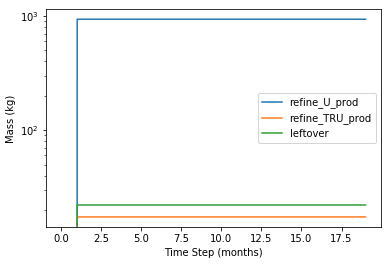
\includegraphics[width=0.65\linewidth]{images/timeseries-prod}
	\caption{Product time series of a simple simulation.}
	\label{fig:timeseries-prod}
\end{figure}



\begin{figure} [h]
	\centering
	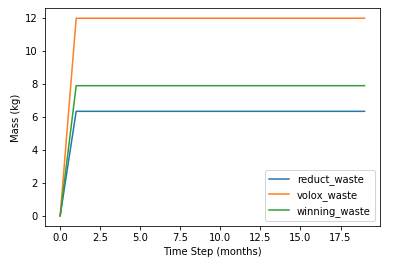
\includegraphics[width=0.65\linewidth]{images/timeseries-waste}
	\caption{Waste time series of a simple simulation.}
	\label{fig:timeseries-waste}
\end{figure}

The above figures \ref{fig:timeseries-prod} and \ref{fig:timeseries-waste} track the shipment of material from the pyre facility to the sink.
Individual waste streams are identified and verify the functionality of each sub-process in this LWR configuration. Since the scenario is run with
constant parameters and number of facilities the transactions are expected to remain constant and the above figures meet this expectation.
In addition to demonstrating sub-process capabilities, material transactions with other Cyclus facilities can also be observed as expected.

\subsection{Isotopic Streams}
\begin{figure} [h]
	\centering
	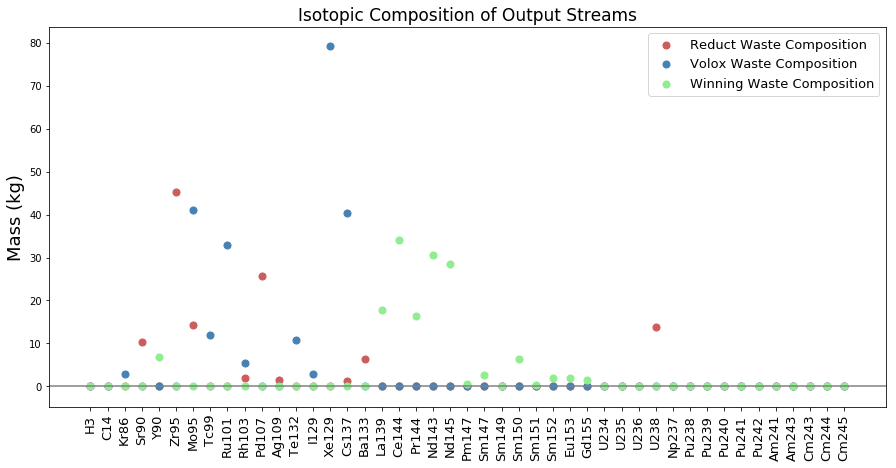
\includegraphics[width=\linewidth]{images/avg-isotope-comp}
	\caption{Isotopic Composition of Average Waste Streams}
	\label{fig:avg-isotope-comp}
\end{figure}

Another key aspect of material transactions is the composition of each shipment. To meet Cyclus standards we must be able to track each isotope for
separation and trading with various facilities. This is done in a couple ways within Pyre, the first being various stream types such as waste or product,
and the second being isotopic composition withing these streams. In Figure \ref{fig:avg-isotope-comp} the 3 waste streams shown in Figure \ref{fig:timeseries-waste}
are compared isotopicaly. We do this comparison to further investigate the performance of each sub-process by identifying the appropriate separation of elements.
We can see that the Electrowinner, shown in green, correctly contains heavier elements such as lanthanides while the Electroreductor, in red, is responsible for the lighter metals
as well as changing oxidation states which is not reflected in these streams.

\subsection{Simple Diversion}
\begin{figure} [h]
	\centering
	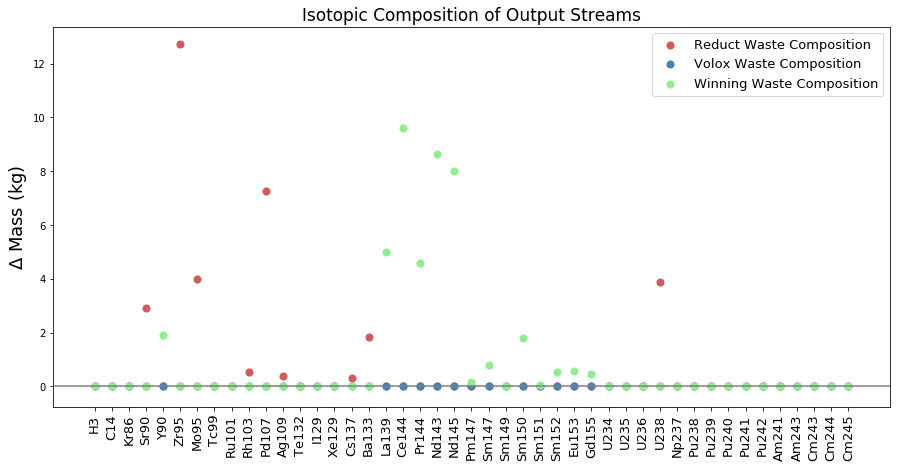
\includegraphics[width=\linewidth]{images/current-isotope-comp}
	\caption{Isotopic Composition of Current Diverted Waste Streams}
	\label{fig:current-isotope-comp}
\end{figure}

\begin{figure} [h]
	\centering
	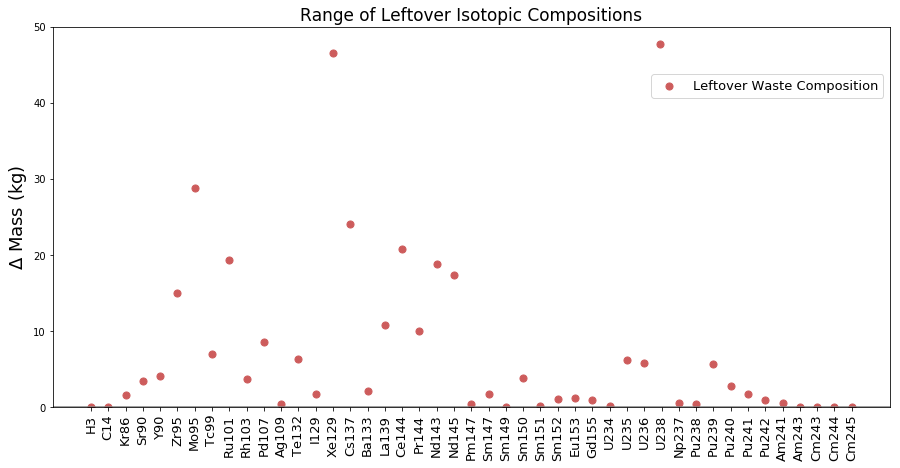
\includegraphics[width=\linewidth]{images/isotopic-comp-range}
	\caption{Range of Isotopic Values for maximum potential diversion.}
	\label{fig:isotopic-range}
\end{figure}

Figures \ref{fig:current-isotope-comp} and \ref{fig:isotopic-range} are used to demonstrate simple diversion scenarios. In particular, the scenario run for Figure
\ref{fig:current-isotope-comp} compares the average case with one of increased power draw. Increasing the power draw of the facility affects sub-process currents.
Separation efficiency of the reductor and winner is improved by increasing the current in the anode resulting in the Material Unaccounted for shown above. Voloxidation stream
is kept on the plot as a validation only appropriate processes are being affected. 

The other diversion scenario explored here is a theoretical maximum diversion scenario in which two scenarios are run: where parameters are set to their maximum and minimum values
respectively. Although an unrealistic scenario since diversion is easily detected, the scenario shows us the worst case scenario and could be used to inform inspection intervals.
Figure \ref{fig:isotopic-range} shows that after the 20 months scenario approximately a significant quantity of plutonium is unaccounted for. As such, inspections would need to occur
at a similar interval, depending on the reported capacity.

\section{US Fuel Cycle}

\begin{figure} [h]
	\centering
	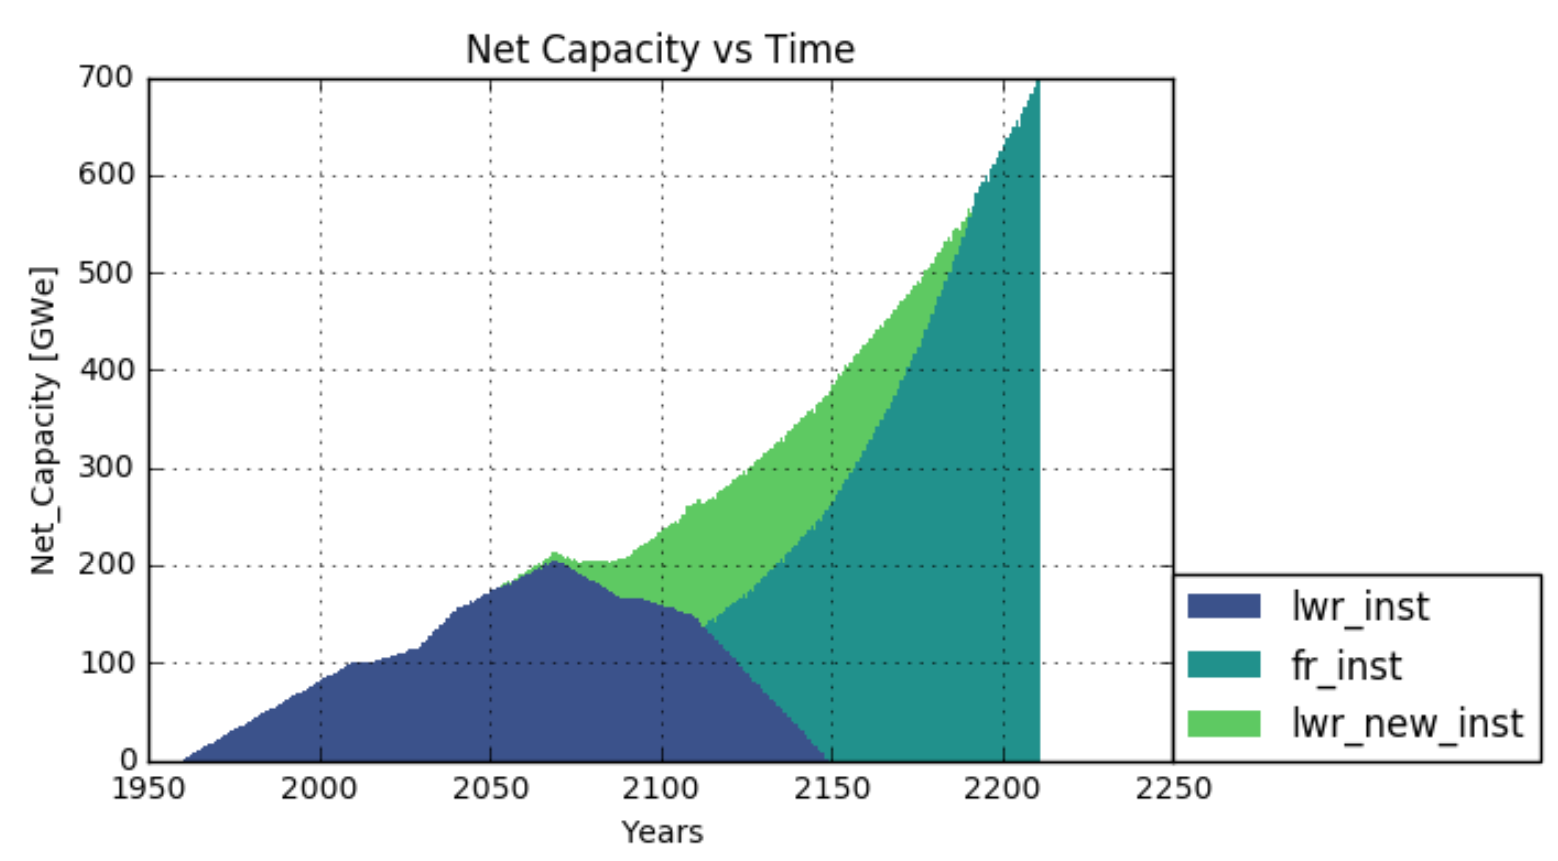
\includegraphics[width=\linewidth]{images/transition-netcap}
	\caption{Net Power Capacity over Time}
	\label{fig:net-cap}
\end{figure}

\begin{figure} [h]
	\centering
	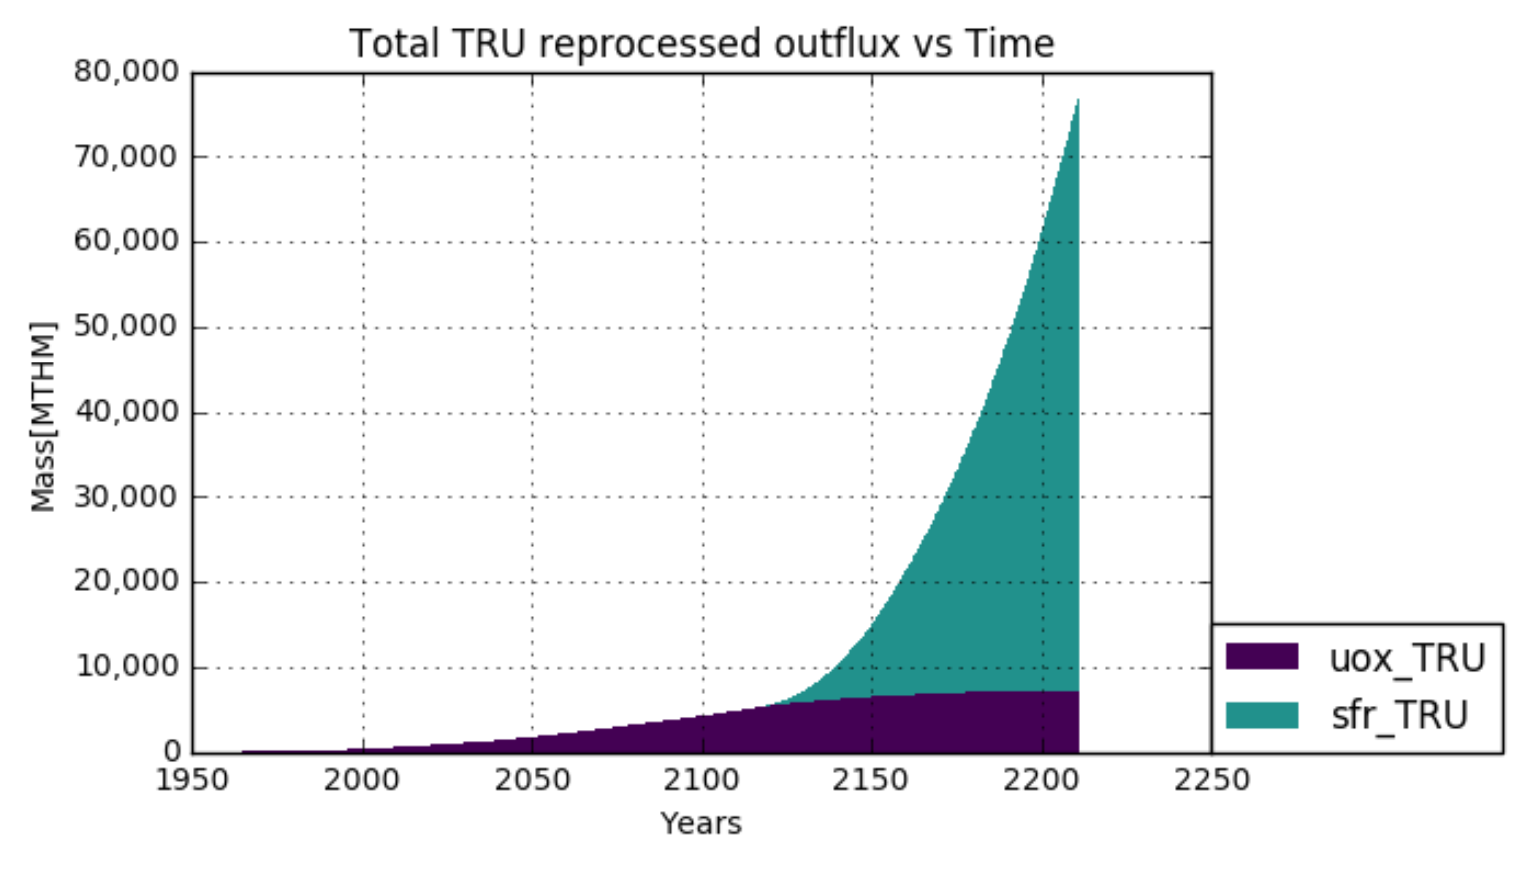
\includegraphics[width=\linewidth]{images/transition-TRUutil}
	\caption{TRU utilization over Time}
	\label{fig:TRU-util}
\end{figure}

\begin{figure}[h]
	\centering
	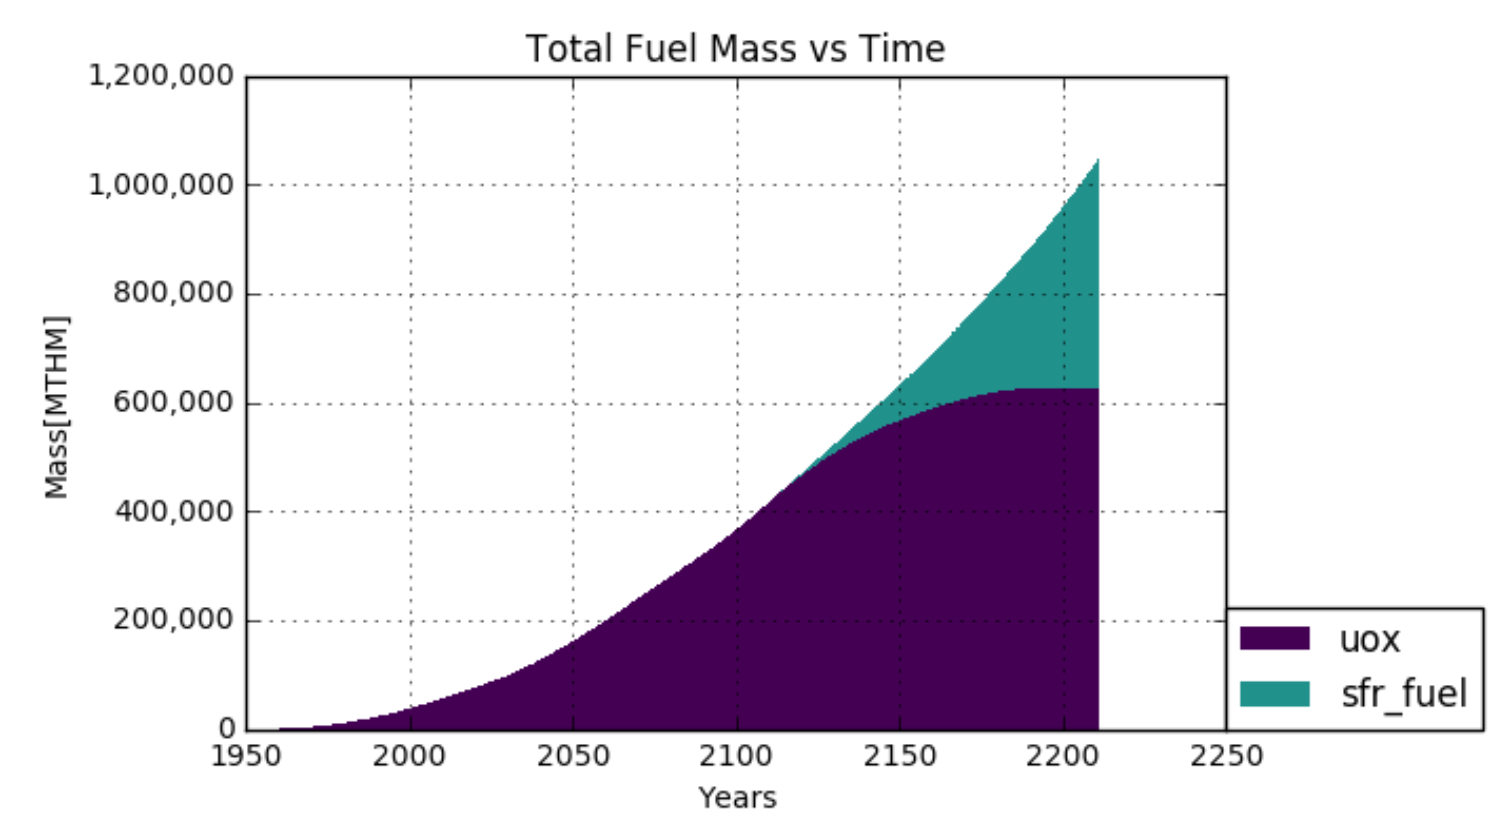
\includegraphics[width=\linewidth]{images/transition-fuelmass}
	\caption{Mass of Fuel Types over Time}
	\label{fig:fuel-mass}
\end{figure}